\documentclass{article}
\usepackage[utf8]{inputenc}

\title{Cosmological Evidences of Dark Matter through the CMB}
\author{Lorenzo Speri}
\date{}

\usepackage{natbib}
\usepackage{graphicx}

\begin{document}

\maketitle


\section{Introduction}
-brief thermal history of the universe and how to get to the cmb and what is it?\\
-practical Motivation for studyinbg the cmb: nice spectrum black body spectrum: physics well know, very intense radiation\\
which info can we get from the cmb: Big bang, maater and energy content of the universe---dark matter is a big part of the matter content it influenced the spectrum  of the CMB ---- so it played a role.\\
-structure of the paper \\



%The recent measurements of the Cosmic Microwave Background (CMB) radiation allowed us to infer the presence of Dark Matter in the Universe. In this summary we will explain qualitatively how the presence of Dark Matter influences the CMB anisotropies.

\section{From the Discovery of the CMB to the Planck mission}
\citep{bucherPhysicsCosmicMicrowave2015}
-discovery of the cmb
-filterng of the images
-different missions






\begin{figure}[h!]
\centering
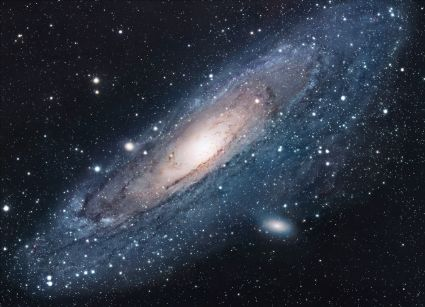
\includegraphics[scale=1.7]{universe}
\caption{The Universe}
\label{fig:universe}
\end{figure}

\section{Conclusion}
nn
\citep{padmanabhanDetectingDarkMatter2005}



\bibliographystyle{plain}
\bibliography{dark}
\end{document}
